\chapter{Assignment: Decision Boundaries}
\label{hw:decision-boundaries}

\marginnote{You can try painting the data yourself or download it from \href{http://file.biolab.si/datasets/decision-boundaries-data.zip}{here}.}

\begin{marginfigure}
    \centering
    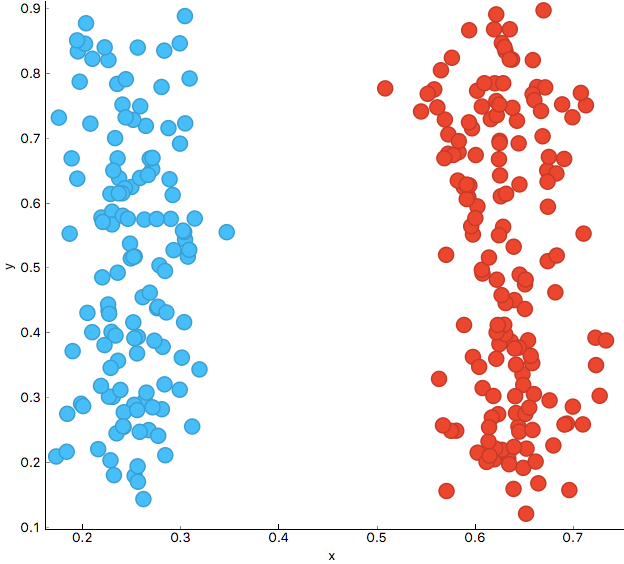
\includegraphics[width=\linewidth]{A.png}
    \caption{$\;$}
\end{marginfigure}

\begin{marginfigure}
    \centering
    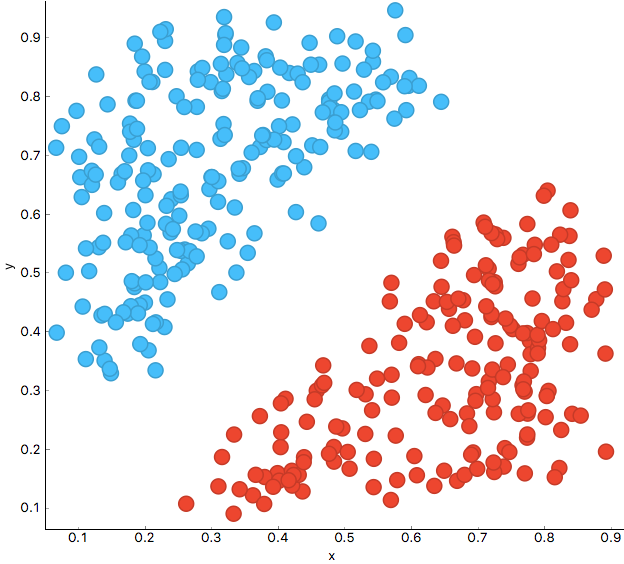
\includegraphics[width=\linewidth]{B.png}
    \caption{$\;$}
\end{marginfigure}

\begin{marginfigure}
    \centering
    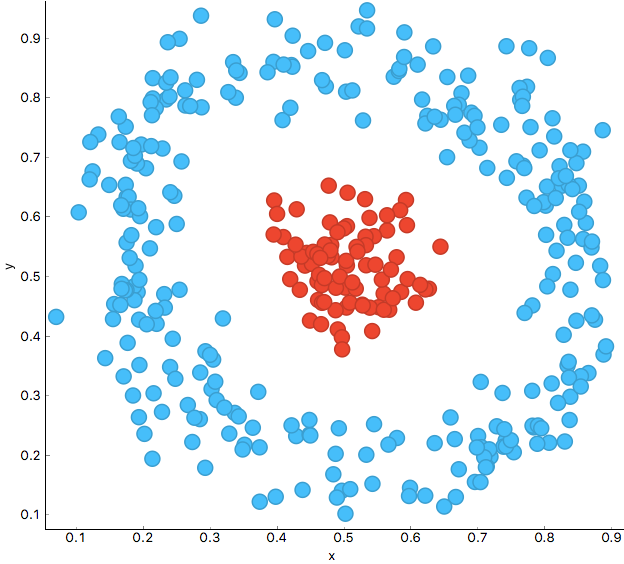
\includegraphics[width=\linewidth]{C.png}
    \caption{$\;$}
\end{marginfigure}

\begin{marginfigure}
    \centering
    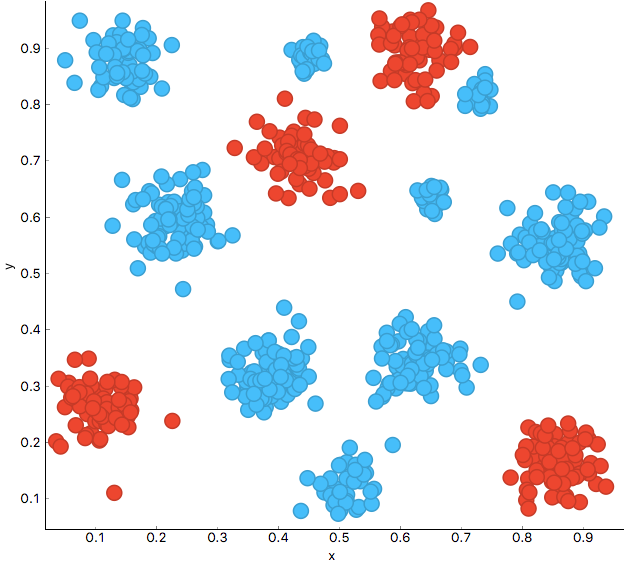
\includegraphics[width=\linewidth]{D.png}
    \caption{$\;$}
\end{marginfigure}

\newthought{Classifiers come in all shapes and sizes.} What we mean by that is that each has its own way of learning from the data, its own strengths and weaknesses. Knowing how classifiers work is crucial for selecting the right algorithm for your task.

\begin{figure}[h]
    \centering
    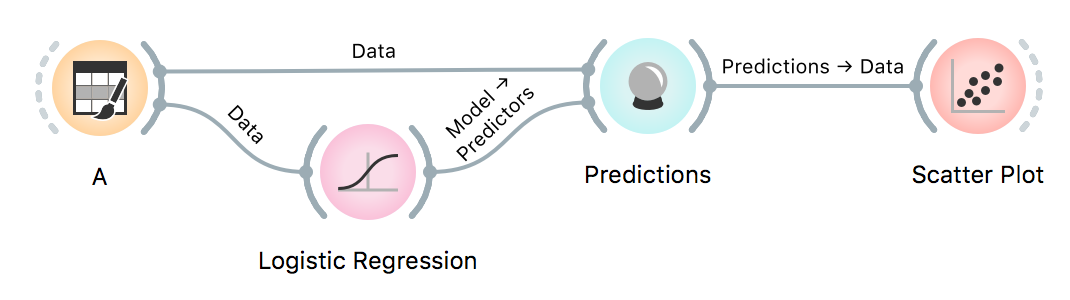
\includegraphics[width=\textwidth]{workflow.png}%
    \caption{$\;$}
  \end{figure}

Try \widget{Tree}, \widget{Logistic Regression}, \widget{SVM}, \widget{Random Forest}, and \widget{kNN} classifiers:
\begin{enumerate}
    \item Which classifiers work well with data set A? Which with B, C, and D?
    \item Which classifier is struggling the most? Which one the least? Why?
    \item Look at the Tree with \widget{Tree Viewer} for data set C. What do you notice?
    \item In the above example, you can separate classes with a single stroke of a pen. Now limit Tree depth by setting \textit{Limit maximal tree depth to} 2, which replicates drawing a single line to separate the classes. What do you notice? What happens, when you increase the depth of the tree?
\end{enumerate}
